\chapter*{General Introduction}
\addstarredchapter{Introduction}

% TODO: fix header text


Metallurgical processes have known a great evolution during the last 60 years. The advancement is attributed to 
research disciplines, like physical metallurgy, which investigated a great deal of solidification-related phenomena.
Today, research in metallurgy focuses on a deeper understanding of the connection between the different physical scales.
Solidification is not only a phase change, but also a complex transformation involving small scales like nucleation, medium scales
like grains growth and large scales like convection in the melt. 
From the nucleation theory to the mechanical behavior of metals, intricate phenomena combine to form defects in the final product. This has been seen in casting processes, such as continuous casting and ingot
casting. Surface and volume porosity, hot tearing and composition heterogeneity are known defects to the casting community.
As far as the current project is concerned, the last defect, also widely known as macrosegregation, is the subject of this thesis.

\comment{ should I add the use of the word "solidification" from google ngram (books) or archiX (articles) ? }

\section*{Casting process}

\section*{Defects}
Undesired effects are inevitable in any industrial process. More importantly, a lot of defects in the casting industry can be disastrous in some situations where the cast product is not serviceable and hence rejected. This leads to a systematic product recycling, i.e. the product is ditched to be reheated, remelted and then cast again. From an economic point view, the operation is expensive timewise and profitwise. Understanding and preventing defects when possible, is thus crucial in the casting industry.
We focus hereafter on the main encountered defects.

\subsection*{Hot tearing}
This defect, also denoted solidification cracking or hot cracking, occurs in the mushy zone at high solid fractions when a failure
or crack appears at specific locations, the hot spots. The temperature range in which the steel is vulnerable to hot tearing is known as the brittleness temperature range (BTR). It corresponds to solid fractions greater than \num{90}\%, with the liquid phase forming a discontinuous film (\red{FIGURE A}). Many factors can cause the failure, but the main origin is a lack of liquid feeding required to compensate for the solidification shrinkage, in the presence of thermal stresses in the mushy region. Therefore, a crack initiates then propagates in the casting (\red{FIGURE B}). 

\subsection*{Porosity}
\url{http://www.afsinc.org/about/content.cfm?ItemNumber=6933} \\
\url{http://en.wikipedia.org/wiki/Casting_defect} \\
Porosity is a void defect formed inside the casting or at the outer surface. It may attributed to two different factors.
Firstly, we speak of \emph{shrinkage porosity}, when a void forms as a result of density differences between the interdendritic liquid and solid
network, the latter being denser than the former. It is basically, the same reason that initiates hot cracks. 
The second factor is the presence of dissolved gaseous phases in the melt. According to \citet{dantzig_solidification_2009}, these gases may be initially in the melt, or created by the reaction between the metal and water found in the air or at trapped in grooves at the molds surface. If the decreasing temperature and pressure drop in the liquid are large enough, the latter becomes supersaturated. Consequently, the nucleation of gaseous phase is triggered (just like when you open a cold bottle of coca-cola!).
\comment{Here goes the porosity figure}

\subsection*{Freckles and segregated channels} 
The intersection between the effects of microsegregation and gravity forces is the origin of freckles. They may appear 
in all casting processes, but are very specific to directional chill casting \citep{giamei_nature_1970}, mainly vertical chill casting. 
\comment{give a more detailed example in chapter 3: e.g. Pb Sn is not like Sn Pb and explain}
Segregation takes place at a medium scale (ranging from the scale of a few dendrites to a few hundreds of them), hence forms "long and narrow trails" as described by \citet{felicelli_simulation_1991}. The segregated channels are frequently formed by small equiaxed grains, probably caused by a uniform temperature
gradient that settles as the channels become richer in solute. They can be observed on the ingot's surface, as well as in the volume (\blue{thèse kohler exemple or article felicelli}).

\subsection*{Macrosegregation}
In principle, macrosegreation stems from the same causes of freckles and segregated channels. However, this defect is characterized by a composition heterogeneity on much larger scale (\red{give scale}). 
\comment{put the Nancy ingot photo and comment it. Also put a photo either from
Beckermann review 2000 or the big review article by rappaz, rohit, beckermann ...}
\comment{DO NOT GIVE ALL THE INFORMATION HERE, REFER TO CHAPTER 1 (details about macrosegregation modelling: miha zalonik Oleron presentation)}

\section*{Industrial Worries}
\textbf{Steel production} has continuously increased over the years to meet the industrial needs. \autoref{fig:steel_production} shows this increase between 1980 and 2013 with a 
clear dominance of the chinese production. Quality constraints have also increased where specific grades of steel are needed in critical applications such as megastructures
in construction and  heavy machinery. Therefore, the presented defects should be avoided as much as possible during the casting process. As such, steelmakers have been investing
in research, with the aim of understanding better the phenomena leading to casting problems, and improve the processes when possible.

\begin{figure}[!h]
\centering
\begin{tikzpicture}
 \pgfkeys{%
    /pgf/number format/set thousands separator = {}}
\begin{axis}
[
	table/col sep=comma,
	smooth, %ybar
	stack plots=y,
	area style,
	enlarge x limits=false,
	legend pos=north west,
	scaled ticks=true,
	xlabel=Year,
	ylabel=Production (tons),
	xticklabel style={/pgf/number format/fixed},
	xtick={1980,1990,2000,2010},
	%x tick label style={rotate=45,anchor=east},
	%width=0.5\textwidth
]
\addplot table [x=Year, y expr=\thisrow{EU}*1000] {Chapter0/Data/steel_production.csv} \closedcycle ;
%\addlegendentry{EU (27)}
\addplot table [x=Year, y expr=\thisrow{China}*1000] {Chapter0/Data/steel_production.csv}\closedcycle;
%\addlegendentry{China}
\addplot table [x=Year, y expr=\thisrow{World}*1000] {Chapter0/Data/steel_production.csv}\closedcycle;
%\addlegendentry{World}
\legend{EU (27), China, World}
\end{axis}
%\addplot table [x expr=\coordindex, y=EU] {Chapter0/Data/steel_production.csv};
\end{tikzpicture}
\caption{Evolution curves of crude steel worldwide production from 1980 to 2013}
\label{fig:steel_production}
\end{figure}

\textbf{Simulation software } dedicated to alloy casting is one of the main research investments undertaken by steelmakers. These tools coming from academic research
are actively used to optimize the process. However, few are the tools that take into account the casting envionment. For instance, the continuous casting process, in
\autoref{fig:cc_process}, is a chain process where the last steps involve rolls, water sprays and other components. A dedicated software is one that can provide the
geometric requirements with suitable meshing capbilities, as well as respond to metallurgical and mechanical requirements, mainly:
\begin{itemize}
\item handling molds and their interaction with the alloy (thermal resistances ...)
\item handling alloy filling and predicting velocity in the liquid and mushy zone
\item handling thermomechanical stresses in the solid
\item handling multicomponent alloys and predicting macrosegregation
\item handling finite solute diffusion in solid phases
\item handling real alloy properties (not just constant thermophysical/thermomechanical properties)
\end{itemize}

These requirements are not met in a single software package. Nevertheless, \thercast is a promising tool that already 
handles a part of the above points. The current thesis developments are done using C++ language as a part of the
in-house code, known as \cimlib. This fully parallel library is the main academic research support for \thercast.
\comment{Add Digonnet reference for Cimlib}

\begin{figure}
	\centering
    %\def\svgwidth{350pt}
	%\import{Chapter0/Graphics/}{cc_process.pdf_tex}
	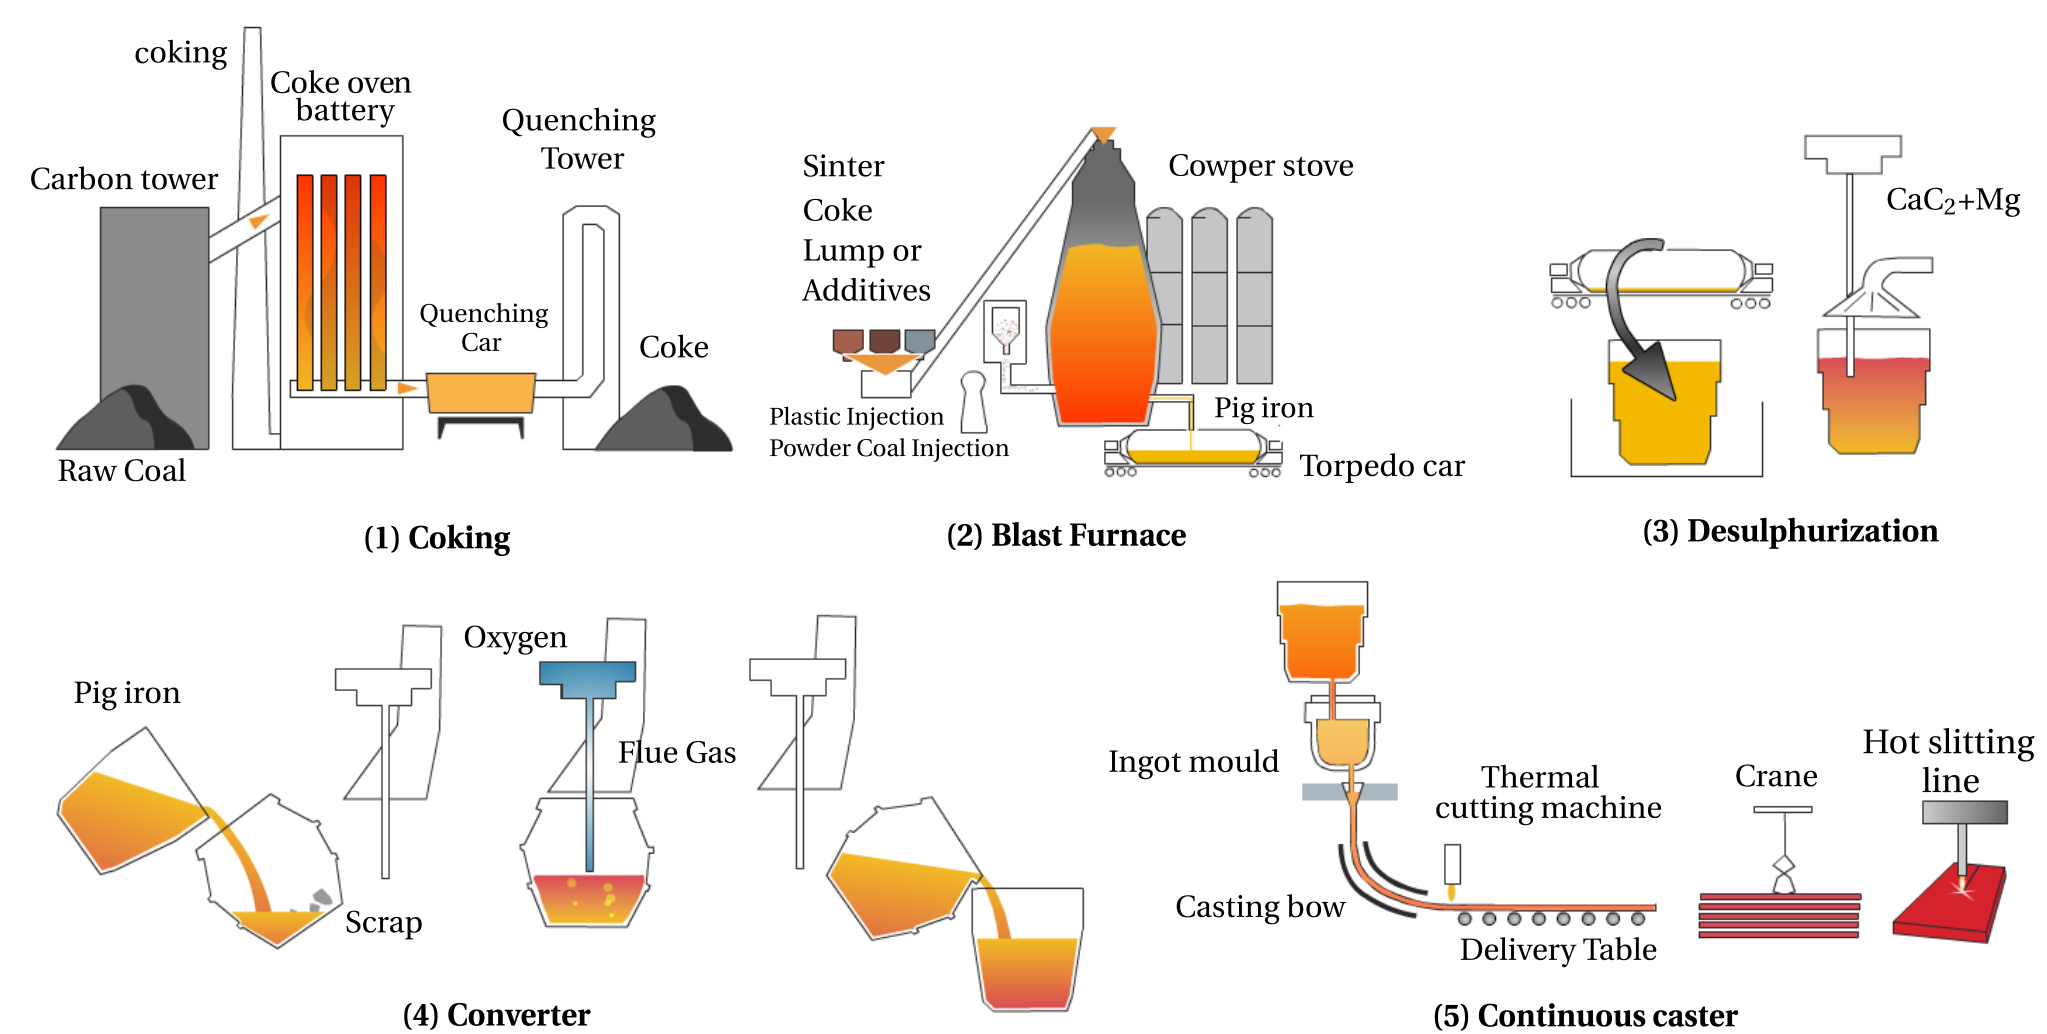
\includegraphics[width=\textwidth]{Chapter0/Graphics/cc_process}
\caption{Main steps in a continuous casting plant}
%source: http://bremen.arcelormittal.com/produktionsablauf_animiert.html?&L=1
\label{fig:cc_process}
\end{figure}


\section*{\ccemlcc project}

Since its foundation in 1975, the European Space Agency (ESA) has been actively committed in the research field.
Their areas of activity cover not only exclusive space applications, but also fundamental science related to 
physics and other disciplines. This thesis is part of the ESA project entitled \ccemlcc, abbreviating
"\textbf{C}hill \textbf{C}ooling for the \textbf{E}lectro-\textbf{M}agnetic \textbf{L}evitator in relation with 
\textbf{C}ontinuous \textbf{C}asting of steel".
The three-year contract from 2011 to 2014 denoted \ccemlcc II, was preceded by an initial project phase, \ccemlcc I,
from 2007 to 2010. The main focus is studying containerless solidification of steel under microgravity conditions. 
Moreover, a chill plate is used to extract heat from the droplet, simulating the effect of the alloy contact with the 
CEMEF contributed to the work by proposing numerical models and simulation tools in 
view of predicting the chill cooling of steel droplets. A first model was developed by \citet{rivaux_simulation_2011} whereas
the present discusses a new model. The experimental work considered various facilities and environments 
to set a droplet of molten alloy in levitation: electromagnetic levitation (EML) for ground-based experiments, microgravity 
in parabolic flight or sounding rockets and last, microgravity condition on-board the International Space Station (ISS)
\comment{DLR droplet EML photo}

\begin{itemize}
\item in what ways does this project tries to alleviate the aforementionned problems ?
The two phases of CCEMLCC, together with the newly coming \ccemlcc III, aim to shape our understanding
of solidification with thermo-mechanical stresses under microgravity conditions.
\item academic and industrial partners and how does each of them contribute actually
\end{itemize}

%\section*{Trying \emph{SIUNITX}}
%Here i wana test the SI units package via the commands \num{.3e45} and the unit \si{\kilo\metre}
%then i wanted to see if we combine both via \SI{.3e45}{\kilo\metre} then finally my personal command
%\SI{231e-4}{\uacceleration} \\
%\SI{231e-4}{\ucomposition} C \\
%\SI{231e-4}{\uvelocity} \\
%\SI{231e-4}{\uconductivity} \\
%\SI{231e-4}{\umasscapacity} \\
%\SI{231e-4}{\uvolumecapacity} \\
%Will it work \num{.3e45}   ,  \num{3.45d-4}   , \numlist{10;30;50;70} ,  \numrange{10}{30}
